%%%%%%%%%%%%%%%%%%%%%%%%%%%%%%%%%%%%%%%%%%%%%%%%%%%%%%%%%%%%%%%%%%%%%%%%
%% Description: Slides propostos para Aula 01 - Apresentacao da
%% disciplina e Conceitos Básicos de Análise de Dados...
%% 
%% Maintainer: Rodrigo Sant'Ana - UNIVALI/GEP
%% Author: Rodrigo Sant'Ana
%% Created: Seg Mar  2 08:34:30 2015 (-0300)
%% Version: 0.0.1
%% Last-Updated: Ter Mar  3 21:28:58 2015 (-0300)
%%           By: Rodrigo Sant'Ana
%% 
%% URL: rodrigosantana.github.io
%% Doc URL: rodrigosantana.github.io
%% 
%% Database info: 
%% 
%%% Commentary: 
%% 
%%% Code:
%%%%%%%%%%%%%%%%%%%%%%%%%%%%%%%%%%%%%%%%%%%%%%%%%%%%%%%%%%%%%%%%%%%%%%%%

\documentclass{bredelebeamer}

%%%%%%%%%%%%%%%%%%%%%%%%%%%%%%%%%%%%%%%%%%%%%%%%%%%%%%%%%%%%%%%%%%%%%%%%
%%% Configuracao da apresentacao...

%%% Titulo da apresentacao
\title[Apresentação da Disciplina]{Apresentação da Disciplina e
  Conceitos Básicos}

%%% Subtitulo da apresentacao, se for necessario
%\subtitle{}

%%% Autor da apresentacao ou trabalho... \inst{num} corresponde ao link
%%% a instituicao que o autor esta vinculado
\author{Rodrigo Sant'Ana\inst{1}}

\institute[Universidade do Vale do Itajaí]
{
  \inst{1}%
  Universidade do Vale do Itajaí - UNIVALI\\
  Centro de Ciências Tecnológicas, da Terra e do Mar - CTTMar\\
  Curso de Engenharia Ambiental e Sanitária - EAS
  }

%%% Periodo do curso...
\date{Março, 2015}

%%% Nao faco ideia onde este comando esta atuando...
\subject{}

\logo{

\includegraphics[scale=0.08]{images/univali.jpg}
}

%%%%%%%%%%%%%%%%%%%%%%%%%%%%%%%%%%%%%%%%%%%%%%%%%%%%%%%%%%%%%%%%%%%%%%%%
%%% Inicio do documento...
\begin{document}

%%% Slide de abertura...
\begin{frame}
  \titlepage
\end{frame}

%%% Slide de summario...
\begin{frame}{Sumário}
  \tableofcontents
\end{frame}

%%% Slide de conteudo - Secao 01...
\section{Plano de Ensino}

\subsection{Objetivo Geral}

\begin{frame}{Apresentação do Plano de Ensino}

\Large{\textbf{\textit{Objetivo Geral}}}

\vspace{1cm}

\textbf{\alert{Fundamentar}} o conhecimento básico de análise de dados
através da aplicação de métodos estatísticos e de inferência que
possibilitem compreender \textbf{\exemple{padrões}} e \emph{hipóteses}
que permeiam o cotidiano de profissionais do meio ambiente.

\end{frame}

\subsection{Unidades e Subunidades}

\begin{frame}{Unidades e Subunidades}

\begin{columns}

\begin{column}{0.5\textwidth}
\begin{block}{Unidade 1 - Análise de Variância}
\begin{itemize}
\item Análise de variância simples
\item Análise de variância para dois fatores 
\end{itemize}
\end{block}

\begin{block}{Unidade 2 - Regressão}
\begin{itemize}
\item Regressão linear simples
\item Regressão linear múltipla
\end{itemize}
\end{block}

\begin{block}{Unidade 3 - Análise de Covariância}
\begin{itemize}
\item Teoria da análise de covariância
\item Aplicações em problemas ambientais
\end{itemize}
\end{block}
\end{column}

\begin{column}{0.5\textwidth}
\begin{block}{Unidade 4 - Estatística Não Paramétrica}
\begin{itemize}
\item Comparação de amostras
\item Relações entre variáveis
\end{itemize}
\end{block}

\begin{block}{Unidade 5 - Análise Multivariada}
\begin{itemize}
\item Abordagem multivariada
\item Métodos multivariados
\end{itemize}
\end{block}
\end{column}

\end{columns}
\end{frame}

\subsection{Estratégias de Ensino e Abordagem}

\begin{frame}{Estratégias de Ensino e Abordagem}

\begin{columns}

\begin{column}{0.5\textwidth}
\boiteviolette{
  Aulas Teóricas
}
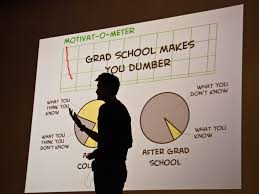
\includegraphics[scale=0.45]{images/teorica.jpg}
\end{column}

\begin{column}{0.5\textwidth}
\boiteorange{
  Aulas Práticas
}
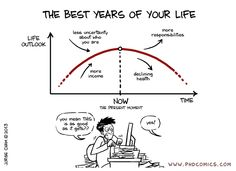
\includegraphics[scale=0.5]{images/pratica.jpg}
\end{column}
\end{columns}

\end{frame}

\begin{frame}{Estratégias de Ensino e Abordagem - Aulas Práticas}

As aulas práticas serão ministradas com auxílio de dois aplicativos
\emph{\textit{Opensource}}...

\vspace{1cm} 

\begin{columns}
\begin{column}{0.5\textwidth}

\includegraphics[scale=0.15]{images/useR-large.png}
\end{column}

\begin{column}{0.5\textwidth}

\includegraphics[scale=0.5]{images/RStudio.png}
\end{column}
\end{columns}

\end{frame}

\begin{frame}{Estratégias de Ensino e Abordagem - Aulas Práticas}

Interface \alert{não tão amigável} para novos usuários!!!

\vspace{.2cm}

\begin{center}
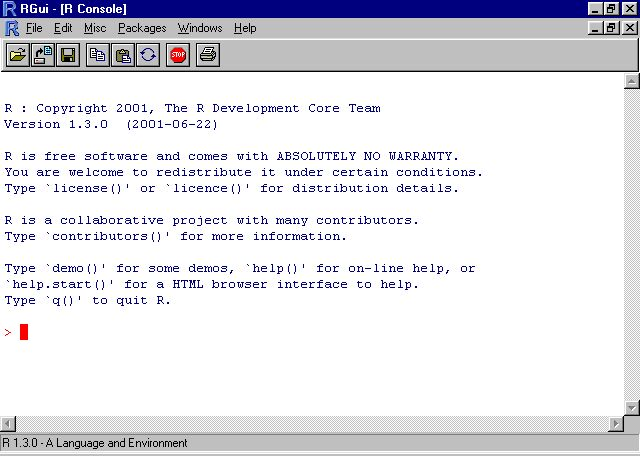
\includegraphics[scale=0.5]{images/R-prompt.jpg}
\end{center}
\end{frame}

\begin{frame}{Estratégias de Ensino e Abordagem - Aulas Práticas}

Interface \emph{um pouco mais amigável} para novos usuários!!!

\vspace{.2cm}

\begin{center}
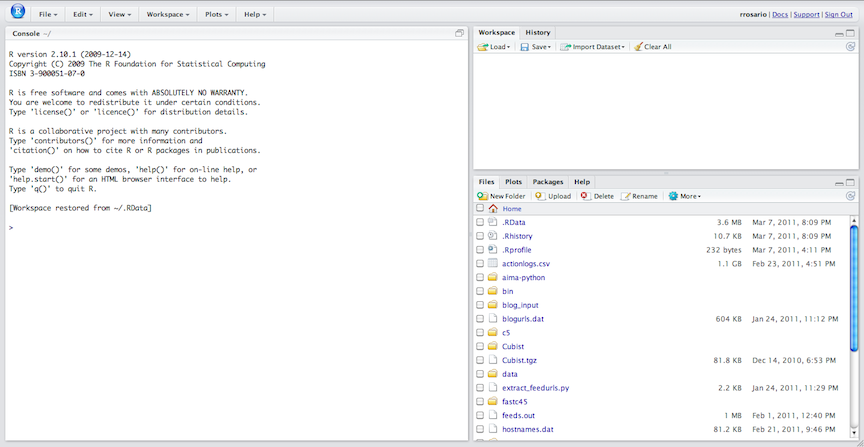
\includegraphics[scale=0.3]{images/rstudio-prompt.png}
\end{center}
\end{frame}

\subsection{Atividades Avaliativas}

\begin{frame}{Atividades Avaliativas}

\begin{alertblock}{M1}
\begin{itemize}
\item[1.] Atividade curricular - ANOVA - 25 de Março (Peso 5,00)
\item[2.] Prova escrita - ANOVA - 08 de Abril (Peso 5,00)
\end{itemize}
\end{alertblock}

\begin{alertblock}{M2}
\begin{itemize}
\item[3.] Estudo de caso - Regressões Lineares - 06 de Maio (Peso 5,00)
\item[4.] Estudo de caso - ANCOVA - 27 de Maio (Peso 5,00)
\end{itemize}
\end{alertblock}

\begin{alertblock}{M3}
\begin{itemize}
\item[5.] Prova prática - Estatística não paramétrica - 17 de junho (Peso 5,00)
\item[6.] Seminário - Análise Multivariada - 01 de julho (Peso 5,00)
\end{itemize}
\end{alertblock}

\end{frame}

\subsection{Observações Gerais}

\begin{frame}{Observações Gerais}

\begin{exampleblock}{Informações do Professor}
Laboratório do Grupo de Estudos Pesqueiros (UNIVALI/GEP), sala 114, 
bloco E2. e-mail: rsantana@univali.br.
Horário de atendimento: sextas-feiras das 14:00 às 17:00, outros dias e
horários podem ser agendados por e-mail.
\end{exampleblock}

\begin{block}{Outras informações}
\begin{itemize}
\item Ausência em atividades avaliativas
\item Uso de celulares em sala de aula
\item Reposição de aulas
\item Aulas práticas - Scripts de aula
\item Semana Acadêmica SAC
\end{itemize}
\end{block}

\end{frame}

\section{Conceitos Básicos}

\begin{frame}{Conceitos Básicos}

\begin{columns}
\begin{column}{0.5\textwidth}
\begin{flushleft}
\begin{itemize}
\item \textbf{\exemple{Visão Geral}}
\item \textbf{\exemple{Definições Importantes}}
\item \textbf{\exemple{Dados}}
\item \textbf{\exemple{Tipos de Dados}}
\item \textbf{\exemple{Senso Crítico}}
\end{itemize}
\end{flushleft}
\end{column}

\begin{column}{0.5\textwidth}

\begin{figure}
\begin{flushleft}
  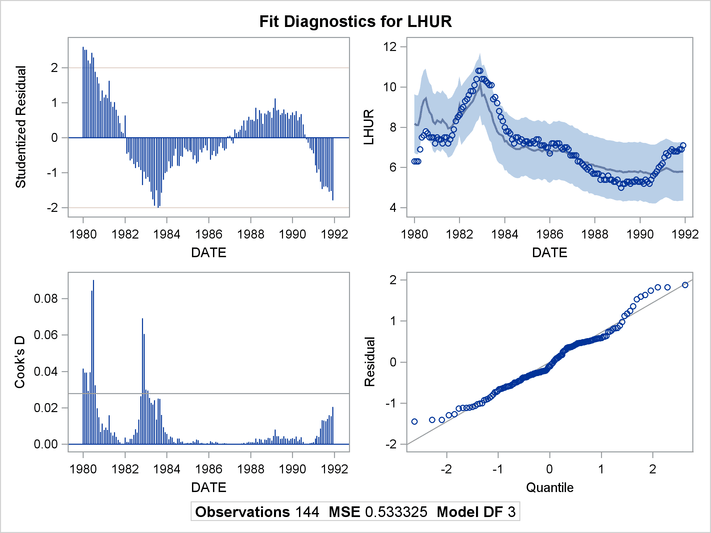
\includegraphics[width=0.5\textwidth]{images/modeldiag.png}
\end{flushleft}
\end{figure}

\begin{figure}
\begin{flushright}
    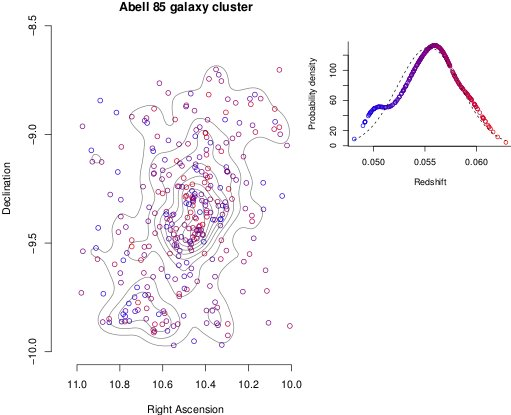
\includegraphics[width=0.5\textwidth]{images/galaxy_density_contours.jpg}
\end{flushright}
\end{figure}

\begin{figure}
\begin{flushleft}
  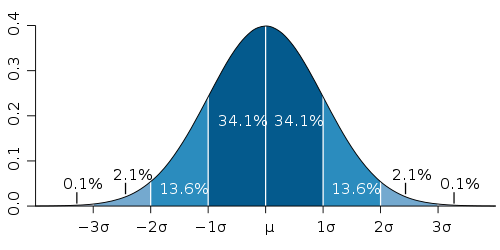
\includegraphics[width=0.5\textwidth]{images/bell_curve.png}
\end{flushleft}
\end{figure}

\end{column}

\end{columns}
\end{frame}

\section{Visão Geral}

\begin{frame}{Visão Geral}
\boiteviolettee{
  ``Ao fazermos uma pesquisa, ou ao utilizarmos algum mecanismo para
  obtenção de informações, um dos objetivos principais é coletar dados
  de uma pequena parte de um determinado grupo de interesse, para assim,
  aprender alguma coisa sobre esse grupo maior.''\\ 
\begin{flushright}
  (Humber Agrelli Andrade, 2008) 
\end{flushright}
}

\begin{center}
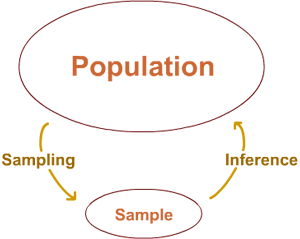
\includegraphics[scale=0.4]{images/population.png}
\end{center}
\end{frame}

\section{Definições Importantes}

\begin{frame}{Definições Importantes}
\begin{columns}
\begin{column}{0.3\textwidth}
\begin{center}
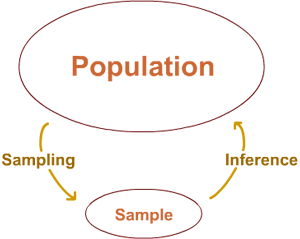
\includegraphics[scale=0.3]{images/population.png}
\end{center}
\end{column}

\begin{column}{0.7\textwidth}
\begin{block}{População}
  \footnotesize{A coleção completa de todos os elementos (escores, indivíduos,
    medidas e outros - ``dados'') a serem estudados, ou melhor, alvos do
    estudo.}
\end{block}

\begin{exampleblock}{Amostragem}
  \footnotesize{Processo ou técnica de seleção de amostra(s) adequadas
    para análise de uma população.}
\end{exampleblock}

\begin{alertblock}{Amostra}
  \footnotesize{Sub-conjunto de membros ou unidades selecionadas da população alvo do
    estudo.}
\end{alertblock}

\begin{block}{Censo}
  \footnotesize{Conjunto de todos os membros ou unidades selecionadas da
  população alvo do estudo.}
\end{block}

\begin{exampleblock}{Dados}
  \footnotesize{Observações que tenham sido coletadas de uma população.}
\end{exampleblock}

%% \begin{exampleblock}{Estatística}
%%   \footnotesize{Métodos utilizados para organização, resumo,
%%   apresentação, análise, interpretação e conclusões pautadas sobre
%%   estes dados.}
%% \end{exampleblock}
\end{column}
\end{columns}
\end{frame}

\begin{frame}{Definições Importantes}

\begin{alertblock}{Parâmetro}
Medida numérica que descreve alguma característica de uma \emph{população}.

\vspace{.1cm}

\begin{center}
\textbf{\emph{População}} \\
\textbf{\emph{$\Updownarrow$}} \\
\textbf{\emph{Parâmetro}} 
\end{center}
\end{alertblock}

\begin{alertblock}{Estatística}
Medida numérica que descreve alguma característica de uma \emph{amostra}.

\vspace{.1cm}

\begin{center}
\textbf{\emph{Amostra}} \\
\textbf{\emph{$\Updownarrow$}} \\
\textbf{\emph{Estatística}} 
\end{center}
\end{alertblock}

\end{frame}

\subsection{Dados}

\begin{frame}{Dados}

\begin{exampleblock}{E o que são \textbf{\exemple{Dados}???}}
$\rightarrow$ Como visto anteriormente, Dados são observações de caráter
\textit{\emph{quantitativo}} e/ou \textbf{\textit{\exemple{qualitativo}}}
relativo a uma determinada população.\\

\vspace{.5cm}

\exemple{Exemplos: medidas de comprimento, peso, sexo, concentrações, respostas
de pesquisas, entre outras.} \\

\vspace{.5cm}

Uma aproximação da compreensão estatística para dados é o conceito de
\exemple{variáveis}. Estas podem ser entendidas como qualquer quantidade,
qualidade, magnitude de um fenômeno/população...\\

\vspace{.5cm}

Assim, convencionalmente, \exemple{Variável} é um elemento representante
de um conjunto de todos os resultados possíveis de um fenômeno. 
\end{exampleblock}

\end{frame}

\subsection{Tipos de Dados/Variáveis}

\begin{frame}{Tipos de Dados/Variáveis}
\begin{center}
\textbf{\alert{Dados ou Variáveis}}
\end{center}

\begin{columns}
\begin{column}{0.5\textwidth}
\begin{alertblock}{\textbf{\emph{Quantitativas}}}
Variáveis quantitativas são números representados por \emph{contagens}
ou \emph{medidas}.
\end{alertblock}

\vspace{.5cm}

\footnotesize{
\textbf{$\rightarrow$} Variáveis \emph{discretas} ou de \emph{contagens}
são provenientes de um processo finito, assumindo geralmente valores
\emph{inteiros}. \\

\begin{flushright}
Exemplo \textbf{\emph{0, 1, 2, 3, ...}}
\end{flushright}
}

\vspace{.5cm}

\footnotesize{
\textbf{$\rightarrow$} Variáveis \emph{contínuas} tratam-se de dados
numéricos que podem assumir \emph{infinitos} valores dentro de um
determinado intervalo. \\

\begin{flushright}
Exemplo \textbf{\emph{0, 0.00001, 0.00002, ..., 0.00003}}
\end{flushright}
}

\vspace{1.15cm}

\end{column}

\begin{column}{0.5\textwidth}
\begin{exampleblock}{\textbf{\exemple{Qualitativas}}}
Variávei qualitativas são qualificações ou definições
\textbf{\exemple{categóricas}} de uma determinada característica. 
\end{exampleblock}

\vspace{0.001cm}

\tiny{
\textbf{$\rightarrow$} Variáveis qualitativas \emph{nominais} são
classes ou símbolos utilizados para identificar grupos de maneira
\textbf{\exemple{não ordenada}}, somente nominal.

\begin{flushright}
Exemplo nomes, respostas ``sim'' ou ``não'', endereços, etc.
\end{flushright}
}

\vspace{0.001cm}

\tiny{
\textbf{$\rightarrow$} Variáveis qualitativas \emph{ordinais} são
classes ou símbolos utilizados para identificar grupos de maneira
\textbf{\exemple{ordenada}}, ou seja, permite classificar o grau
de intensidade relativo de uma resposta.

\begin{flushright}
Exemplo avaliações de perfil em ruim, médio e bom.
\end{flushright}
}

\vspace{0.001cm}

\tiny{
\textbf{$\rightarrow$} Variáveis qualitativas \emph{intervalar} se
assemelham às variáveis ordinais, porém pode-se determinar as diferenças
entre classes. No entanto, \textbf{\exemple{não assumem um zero
    absoluto.}}

\begin{flushright}
Exemplo anos - 2000, 1900, 1000. 
\end{flushright}
}

\vspace{0.001cm}

\tiny{
\textbf{$\rightarrow$} Variáveis qualitativas \emph{racionais} se
assemelham às variáveis intervalares, porém \textbf{\exemple{incluem o
    zero natural como valor inicial}}.

\begin{flushright}
Exemplo Quantidade de amônia nos oceanos, onde o 0 indica inexistência.
\end{flushright}
}

\end{column}
\end{columns}

\end{frame}

\begin{frame}{Tabela - Tipos de Dados}

\exemple{Qual cada tipo de variável e sua subclassificação?}

\vspace{0.5cm}

\begin{tcolorbox}[tabvert,tabularx={X||Y|Y|Y|Y||Y}, boxrule=0.5pt, 
title = Tabela com dados hipotéticos - Monitoramento de um determinado Rio]
Mês       & O$^2$ \tiny{(mgL$^-1$)} & Número de espécies &  Qualidade do
ambiente & Fluxo de corrente \tiny{(m/s)} & Densidade de algas \tiny{(g)} \\\hline\hline
Janeiro   & 10,00 & 20 &  Ruim   &  40 - 50   & 100,20 \\\hline
Fevereiro & 12,00 & 30 &  Médio   & 40 - 52 & 140.10 \\\hline
Março     & 11,00 & 25 &  Boa   &  20 - 25 & 180.40 \\\hline
Abril     & 9,00 & 3 & Péssima & 100 - 120 & 420.60
\end{tcolorbox}

\end{frame}

\subsection{Senso Crítico}

\begin{frame}{Senso Crítico}
\begin{itemize}
\item O sucesso em cursos introdutórios de estatística ou análise de
  dados tipicamente está mais vinculado à capacidade \emph{Crítica} do
  aluno que a habilidade matemática do mesmo.

\item Lembrem-se disto!!
\end{itemize}
\end{frame}


\begin{frame}
\exemple{A capacidade analítica de um pesquisador, técnico,
  profissional, é a grande chave para o sucesso do mesmo em meio ao
  mundo em que vivemos hoje. A informação está em todo lugar, a
  limitação agora esta na capacidade de lidar com ela.}
\end{frame}


\end{document}

%%%%%%%%%%%%%%%%%%%%%%%%%%%%%%%%%%%%%%%%%%%%%%%%%%%%%%%%%%%%%%%%%%%%%%%%
%% 
%% The MIT License (MIT)
%% 
%% Copyright (c) 2014 Rodrigo Sant'Ana
%% 
%% Permission is hereby granted, free of charge, to any person 
%% obtaining a copy of this software and associated documentation 
%% files (the 'Software'), to deal in the Software without 
%% restriction, including without limitation the rights to use, 
%% copy, modify, merge, publish, distribute, sublicense, and/or 
%% sell copies of the Software, and to permit persons to whom the 
%% Software is furnished to do so, subject to the following 
%% conditions: 
%% 
%% The above copyright notice and this permission notice shall be 
%% included in all copies or substantial portions of the Software.
%% 
%% THE SOFTWARE IS PROVIDED 'AS IS', WITHOUT WARRANTY OF ANY KIND, 
%% EXPRESS OR IMPLIED, INCLUDING BUT NOT LIMITED TO THE WARRANTIES 
%% OF MERCHANTABILITY, FITNESS FOR A PARTICULAR PURPOSE AND
%% NONINFRINGEMENT. IN NO EVENT SHALL THE AUTHORS OR COPYRIGHT HOLDERS 
%% BE LIABLE FOR ANY CLAIM, DAMAGES OR OTHER LIABILITY, WHETHER IN AN 
%% ACTION OF CONTRACT, TORT OR OTHERWISE, ARISING FROM, OUT OF OR IN 
%% CONNECTION WITH THE SOFTWARE OR THE USE OR OTHER DEALINGS IN THE 
%% SOFTWARE.
%% 
%%%%%%%%%%%%%%%%%%%%%%%%%%%%%%%%%%%%%%%%%%%%%%%%%%%%%%%%%%%%%%%%%%%%%%%%
